\documentclass{article}\usepackage{graphicx, color}
%% maxwidth is the original width if it is less than linewidth
%% otherwise use linewidth (to make sure the graphics do not exceed the margin)
\makeatletter
\def\maxwidth{ %
  \ifdim\Gin@nat@width>\linewidth
    \linewidth
  \else
    \Gin@nat@width
  \fi
}
\makeatother

\definecolor{fgcolor}{rgb}{0.2, 0.2, 0.2}
\newcommand{\hlnumber}[1]{\textcolor[rgb]{0,0,0}{#1}}%
\newcommand{\hlfunctioncall}[1]{\textcolor[rgb]{0.501960784313725,0,0.329411764705882}{\textbf{#1}}}%
\newcommand{\hlstring}[1]{\textcolor[rgb]{0.6,0.6,1}{#1}}%
\newcommand{\hlkeyword}[1]{\textcolor[rgb]{0,0,0}{\textbf{#1}}}%
\newcommand{\hlargument}[1]{\textcolor[rgb]{0.690196078431373,0.250980392156863,0.0196078431372549}{#1}}%
\newcommand{\hlcomment}[1]{\textcolor[rgb]{0.180392156862745,0.6,0.341176470588235}{#1}}%
\newcommand{\hlroxygencomment}[1]{\textcolor[rgb]{0.43921568627451,0.47843137254902,0.701960784313725}{#1}}%
\newcommand{\hlformalargs}[1]{\textcolor[rgb]{0.690196078431373,0.250980392156863,0.0196078431372549}{#1}}%
\newcommand{\hleqformalargs}[1]{\textcolor[rgb]{0.690196078431373,0.250980392156863,0.0196078431372549}{#1}}%
\newcommand{\hlassignement}[1]{\textcolor[rgb]{0,0,0}{\textbf{#1}}}%
\newcommand{\hlpackage}[1]{\textcolor[rgb]{0.588235294117647,0.709803921568627,0.145098039215686}{#1}}%
\newcommand{\hlslot}[1]{\textit{#1}}%
\newcommand{\hlsymbol}[1]{\textcolor[rgb]{0,0,0}{#1}}%
\newcommand{\hlprompt}[1]{\textcolor[rgb]{0.2,0.2,0.2}{#1}}%

\usepackage{framed}
\makeatletter
\newenvironment{kframe}{%
 \def\at@end@of@kframe{}%
 \ifinner\ifhmode%
  \def\at@end@of@kframe{\end{minipage}}%
  \begin{minipage}{\columnwidth}%
 \fi\fi%
 \def\FrameCommand##1{\hskip\@totalleftmargin \hskip-\fboxsep
 \colorbox{shadecolor}{##1}\hskip-\fboxsep
     % There is no \\@totalrightmargin, so:
     \hskip-\linewidth \hskip-\@totalleftmargin \hskip\columnwidth}%
 \MakeFramed {\advance\hsize-\width
   \@totalleftmargin\z@ \linewidth\hsize
   \@setminipage}}%
 {\par\unskip\endMakeFramed%
 \at@end@of@kframe}
\makeatother

\definecolor{shadecolor}{rgb}{.97, .97, .97}
\definecolor{messagecolor}{rgb}{0, 0, 0}
\definecolor{warningcolor}{rgb}{1, 0, 1}
\definecolor{errorcolor}{rgb}{1, 0, 0}
\newenvironment{knitrout}{}{} % an empty environment to be redefined in TeX

\usepackage{alltt}

\usepackage{xltxtra} %% For XeTeX font commands
\usepackage[includeheadfoot, margin = 0.5in]{geometry} %% Margins
\usepackage{hyperref}
\usepackage{graphicx} 
\usepackage{sectsty} %% Change format (font) of section headers
\usepackage{tikz}    %% Graphics for banner
\usepackage{parskip} %% Lines between paragraphs, no indentation
\usepackage{booktabs} %% Pretty up the tables
\usepackage{xcolor}

%% Colors
\definecolor{pocDGreen}{HTML}{788172}
\definecolor{pocLGreen}{HTML}{A2B69A}
\definecolor{pocDBlue}{HTML}{3B6E8F}
\definecolor{pocLBlue}{HTML}{A3DCE6}
\definecolor{pocPurple}{HTML}{A784B4}

%% Fonts
\setmainfont{Frutiger LT Std 55 Roman}
\allsectionsfont{\fontspec{Archer}}

\usepackage{fancyhdr} %% Header and Footer formatting
\pagestyle{fancy}

%% Hyperlinks, PDF properties
\hypersetup{
    pdftitle = {POC County Report},
    pdfauthor = {Partners for Our Children},
    pdfcreator = {Gregor Passolt},
    pdfproducer = {Gregor Passolt},
    hidelinks,
    unicode = true
}

%%% Header
\renewcommand{\sectionmark}[1]{\markboth{\MakeUppercase{#1}}{\MakeUppercase{#1}}}
\fancyhf{}
\renewcommand{\headrulewidth}{0.5pt}
\renewcommand{\headrule}{\hbox to\headwidth{%
\color{pocDGreen}\leaders\hrule height \headrulewidth\hfill}}
\rhead{\color{pocDGreen} \leftmark}

%%% Footer
\lfoot{\color{pocDGreen} \href{http://www.partnersforourchildren.org}{www.partnersforourchildren.org}}
\rfoot{\color{pocDGreen} \thepage}
\renewcommand{\footrulewidth}{0.5pt}
\renewcommand{\footrule}{\hbox to\headwidth{\color{pocDGreen}\leaders\hrule height \footrulewidth\hfill}}
\IfFileExists{upquote.sty}{\usepackage{upquote}}{}

\begin{document}






\lhead{\color{pocDGreen} Pierce County Report}
\thispagestyle{empty} %% No header/footer on first page

\begin{tikzpicture}[x=1in, y=1in]

    %%    Set up constants
    \def\banX{\textwidth}
    \def\banY{2in}
    \def\stripeHeight{0.5in}
    \def\stripeYpos{0.55in} %% From top
    \def\triX{0.25in}
    \def\triY{0.15in}
    \def\logoInsetX{0.7in}
    \def\logoInsetY{18pt}
    
    %% Draw Background Geomety
    \filldraw[pocLGreen] (0, 0) rectangle ++(\banX, \banY);
    \filldraw[pocDGreen] (0, \banY - \stripeYpos) rectangle ++(\banX + \triX, - \stripeHeight);
    \filldraw[fill=pocLGreen, draw=pocDGreen, join=bevel, thick]
        (\banX, \banY - \stripeYpos - \stripeHeight) -- ++(\triX, 0) -- ++(-\triX, -\triY) -- cycle;
    
    %% Above-stripe Text
    \node[pocDBlue, below left = 6pt, align = right] at (\banX, \banY)
        {\textbf{Automated County Report}\\\textbf{Generated \today}};
    \node at (\logoInsetX, \banY - \logoInsetY)
        {
\includegraphics[height=0.3in]{pocLogoSmall}};
    
    %% Stripe Text
    \node[right = 6pt, white] at (0, \banY - \stripeYpos - \stripeHeight + 16pt)
        {\fontspec{Archer}\Huge{Focus on Pierce County}};
    
    %% Below Stripe Text
    \node[below right = 6pt, pocDBlue, align = left, text width = \textwidth - 12pt]
        at (0, \banY - \stripeYpos - \stripeHeight - 3pt) {
        This is a draft version of Partners for Our Children's automatically generated county report. 
		The reports will be generated for every county; this sample report focuses  on Pierce County.
        
        Safety measures. Well-Being measures.
        
        \textbf{Note:} Please excuse any awkward spacing and pagebreaks. This report was created by a computer. 
    };
    
\end{tikzpicture}

\section*{Overview}

This Focus on Pierce County report mirrors the structure of the Child Well-Being Data Portal.  If you are viewing this document on an Internet-connected device, you can click on the titles to visit the corresponding sections of the Data Portal.
The Department of Social and Health Services (DSHS) divides Washington State into three regions.Pierce County is in Region 3. Other counties in Region 3 are: Clallam, Clark, Cowlitz, Grays Harbor, Jefferson, Kitsap, Lewis, Mason, Pacific, Pierce, Skamania, Thurston and Wahkiakum Counties.

As is done on the Data Portal, this report geographically categorizes Investigations \& Assessments and In-Home Services offices by office groups and Out-of-Home Care by counties. This is necessitated by the level of detail provided in data extracts from Children's Administration: in many cases a single office serves multiple counties but our data for Investigations \& Assessments and for In-Home Services specify only the office.

The two \emph{County Focus} sections for Investigations \& Assessments and In-Home Services display quarterly point-in-time (i.e., first day of the quarter) trend data for each DCFS office/office group in Pierce County. The \emph{County Focus} section for Out-of-Home Care shows quarterly point-in-time trend data for the entire county.

Two \emph{Regional Context} sections feature "dotplots" that compare rates of Investigations and Assessments and In-Home Services per 1,000 households for all office/office groups in Pierce County. A \emph{Regional Context} section also provides a dotplot that compares rates of out-of-home care per 1,000 children for each county in Region 3. Washington State is also included in the dotplots to give context to the rates presented by office or county.  \href{http://www.partnersforourchildren.org/publications/counts-vs-rates}{Technical Bulletin 3: Counts vs. Rates} for more information.

Table 1 provides relevant, comparative Census data for Pierce County and Washington State. Census data on the total population and the number of children under 18 years of age are used in the calculation of the rates in the \emph{Regional Context} sections below.

% latex table generated in R 3.0.0 by xtable 1.7-1 package
% Tue Apr 23 11:28:51 2013
\begin{tabular}{rll}
  \toprule
 & Pierce County & Washington State \\ 
  \midrule
Total population (2012) & 811,681 & 6,897,012 \\ 
  Percent change in population (2010 to 2012) & 2.1\% & 2.6\% \\ 
  Population under 5 years & 6.9\% & 6.5\% \\ 
  Population under 18 years & 24.3\% & 23.2\% \\ 
  Population: White alone & 77.3\% & 82.0\% \\ 
  Population: Black alone & 7.1\% & 3.8\% \\ 
  Population: American Indian/Alaska Native alone & 1.6\% & 1.8\% \\ 
  Population: Asian alone & 6.2\% & 7.5\% \\ 
  Population: Native Hawaiian/Other Pacific Islander alone & 1.4\% & 0.7\% \\ 
  Population: Multiracial & 6.4\% & 4.3\% \\ 
  Population: Hispanic or Latino Origin & 9.4\% & 11.6\% \\ 
  Population: Not Hispanic, White alone & 70.1\% & 72.1\% \\ 
  Language: Speaking language other than English at home & 14.0\% & 17.8\% \\ 
  Education: High school graduate (age $>$25) & 90.1\% & 89.8\% \\ 
  Average household size & 2.6 & 2.5 \\ 
  People below poverty line (all ages) & 11.6\% & 12.5\% \\ 
  Land area (square miles) & 1,669.5 & 66,455.5 \\ 
  Population per square mile & 476.3 & 101.2 \\ 
   \bottomrule
\end{tabular}



\section{\href{http://www.partnersforourchildren.org//child-well-being/visualizations/investigations-assessments/trends}
{Investigations \& Assessments}}
When professionals and community members report suspected instances of child abuse or neglect to the child welfare system, some of the reports are investigated, some are assessed only (e.g., Family Reconciliation Services), and some \emph{screened out} because the information reported (if true) does not meet the statutory definition of child abuse or neglect and there is no need for an assessment.

The measurements in this section provide an overview of the changes over time in the number of the Washington State households who have received investigations and/or assessments.


\subsection{\href{http://www.partnersforourchildren.org//child-well-being/visualizations/investigations-assessments/trends}
{Investigations \& Assessments:} Pierce County Focus}
Graphs below indicate recent trends in Investigations \& Assessments for the two DCFS offices/office groups in
Pierce County. Data are presented using "unduplicated counts." See \href{http://www.partnersforourchildren.org/publications/using-different-count-types-data-portal}{Technical Bulletin 3: Counts vs. Rates} for more information.
\nopagebreak[4]
\begin{knitrout}
\definecolor{shadecolor}{rgb}{0.969, 0.969, 0.969}\color{fgcolor}

{\centering 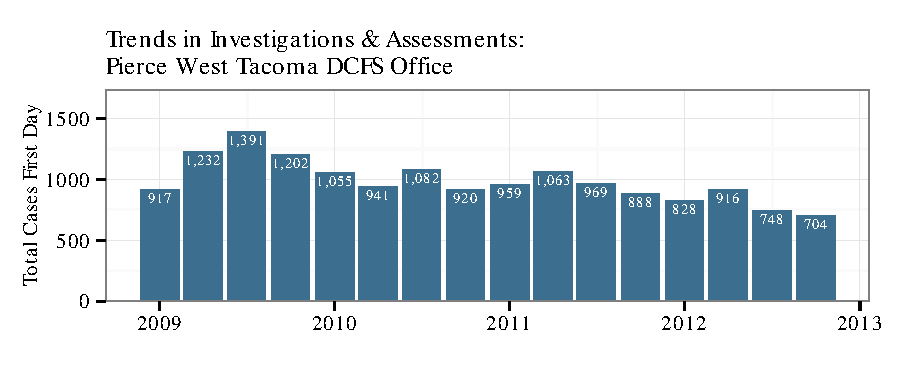
\includegraphics[width=\maxwidth]{figure/ia_focus1} 
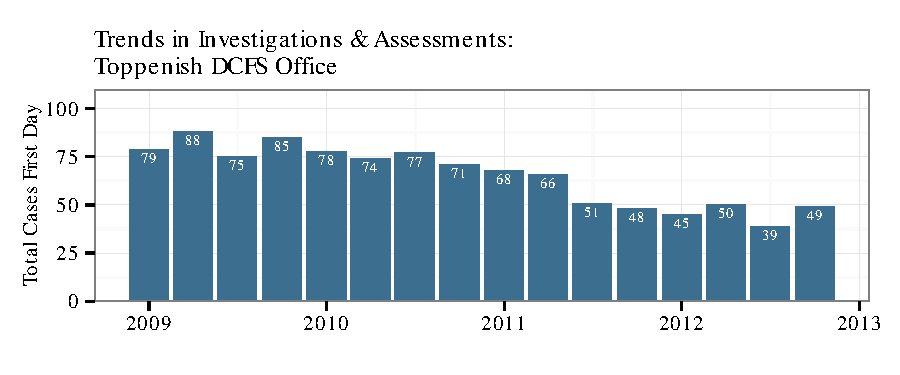
\includegraphics[width=\maxwidth]{figure/ia_focus2} 

}



\end{knitrout}




\subsection{
    \href{http://www.partnersforourchildren.org//child-well-being/visualizations/investigations-assessments/trends}
    {Investigations \& Assessment: Regional Context}}
To give context to the trend data above, this plot shows the rate of Investigations \& Assessments (as a rate per 1,000 households) for quarter 4, of 2012 for Region 3.
\nopagebreak[4]
\begin{knitrout}
\definecolor{shadecolor}{rgb}{0.969, 0.969, 0.969}\color{fgcolor}

{\centering 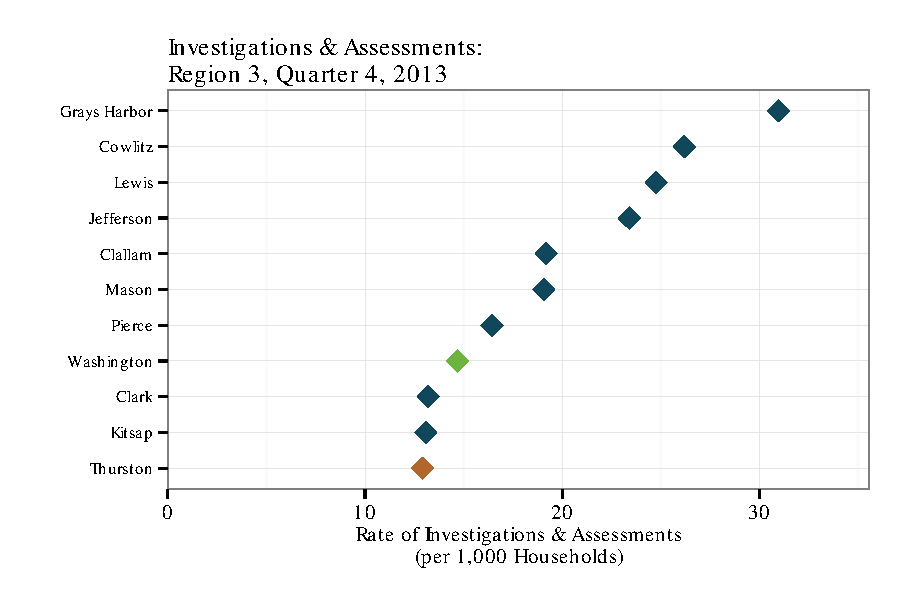
\includegraphics[width=\maxwidth]{figure/ia_context} 

}



\end{knitrout}



%%%%%%%%%%%%%%%%%%%%%%%%%%%%%%%%%%%%%%%%%%%%%%%%
\section{\href{http://www.partnersforourchildren.org/child-well-being/visualizations/home-services/trends}
    {In-Home Services}
}
When an investigation or assessment identifies threats to a child's safety, social workers will first determine if the child can be kept safely at home through a safety plan. If so, the family and child may be provided with various services that range from concrete support (e.g., food, appliance repair, etc.) to referrals to community services (e.g., drug and alcohol assessments, etc.).

The measurements in this section provide an overview of the population of families receiving in-home services and how the population of families has changed over time.


\subsection{\href{http://www.partnersforourchildren.org/child-well-being/visualizations/home-services/trends}
    {In-Home Services: Pierce County Focus}
}
These graphs show the recent trends in In-Home Services for the two DCFS offices in
Pierce County. Data are presented using "unduplicated counts." See \hyperref{http://www.partnersforourchildren.org/publications/using-different-count-types-data-portal}{Technical Bulletin: Count Types} for more information.
\nopagebreak[4]
\begin{knitrout}
\definecolor{shadecolor}{rgb}{0.969, 0.969, 0.969}\color{fgcolor}

{\centering 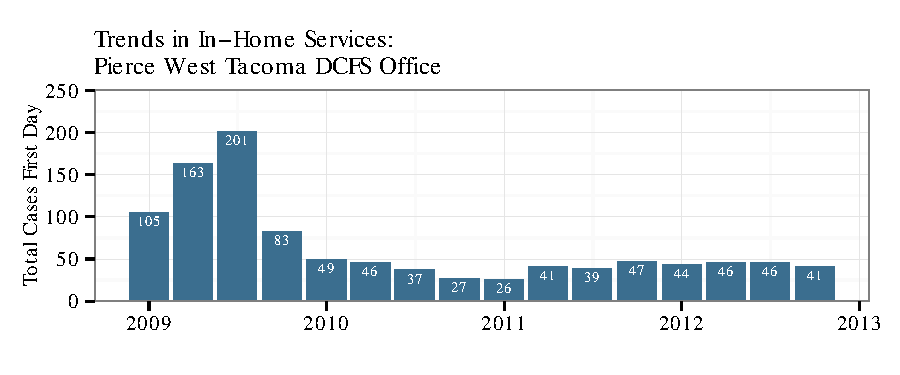
\includegraphics[width=\maxwidth]{figure/ihs_focus1} 
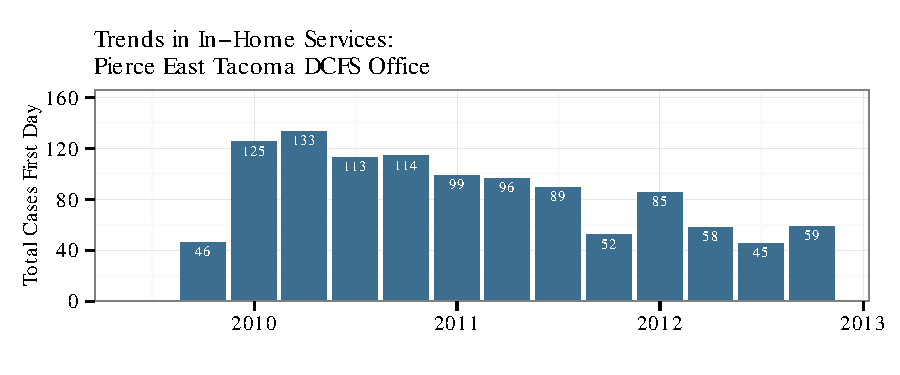
\includegraphics[width=\maxwidth]{figure/ihs_focus2} 

}



\end{knitrout}




\subsection{\href{http://www.partnersforourchildren.org/child-well-being/visualizations/home-services/trends}
    {In-Home Services: Regional Context}
}
To give context to the trend data above, this plot shows the rate of In-Home Services (as a rate per 1,000 households)for quarter 4, 2012 for Region 3.
\nopagebreak[4]
\begin{knitrout}
\definecolor{shadecolor}{rgb}{0.969, 0.969, 0.969}\color{fgcolor}

{\centering 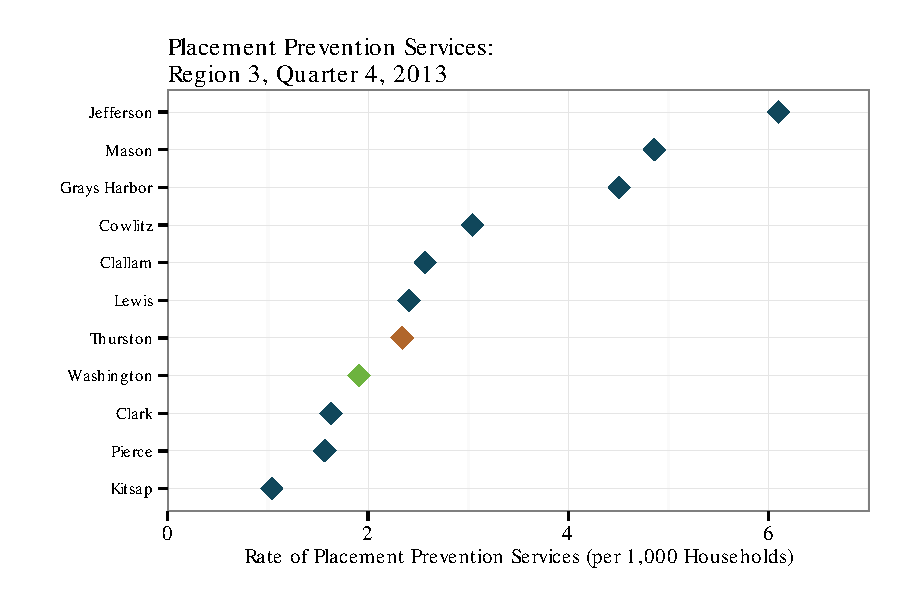
\includegraphics[width=\maxwidth]{figure/ihs_context} 

}



\end{knitrout}



\subsection{\href{http://www.partnersforourchildren.org/child-well-being/visualizations/home-services/safety}
    {In-Home Services: Safety}
}
Sometimes the services provided to families through in-home services do not adequately address the issues identified during the investigation. Other times, new issues are raised during the course of an in-home services case. Either way, when the social worker decides that it is not possible for the child to remain safely in their home steps will be taken to place the child in out-of-home care.

The measurements in Table 2 identify placement into out-of-home care among families and their children who have received in-home services for one year and for two years. If the in-home services are completed effectively, and/or circumstances become such that the child can remain in-home safely, there should be no need to place the child in out-of-home care. Thus, in general, the lower percentages indicate better outcomes.


%%%%%%%%%%%%%%%%%%%%%%%%%%%%%%%%%%%%%%%%%%%%%%%%%
\section{\href{http://www.partnersforourchildren.org/child-well-being/visualizations/out-home-care/trends}
    {Out-of-Home Care}
}
When children cannot remain safely in their home, they are placed in out-of-home care. Once a child is placed in out-of-home care, the child welfare system works to find a safe and permanent home for the child. Most children ultimately reunify with their parents after the safety threats have been controlled. However, some children exit to other permanency outcomes (e.g., adoption, guardianship, etc.).

The measurements in this section provide an overview of the changes over time in the number of the children who have been placed in out-of-home care.


\subsection{\href{http://www.partnersforourchildren.org/child-well-being/visualizations/out-home-care/trends}
 {Out-of-Home Care: Pierce County Focus}
}
This graph shows the recent trends in Out-of-Home Care for
Pierce County. Most counties maintain a relatively stable out-of-home care population; note, however, that when percentages are calculated, smaller counties can seem more volatile. Data are presented using �unduplicated counts.� See Technical Bulletin 3: Counts vs. Rates (add hyperlink) for more information. 
\nopagebreak[4]
\begin{knitrout}
\definecolor{shadecolor}{rgb}{0.969, 0.969, 0.969}\color{fgcolor}

{\centering 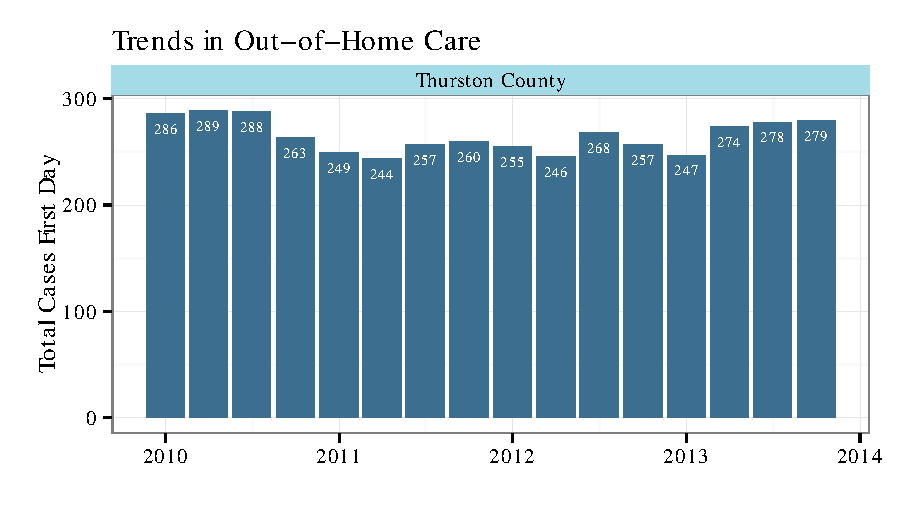
\includegraphics[width=\maxwidth]{figure/ooh_focus} 

}



\end{knitrout}


\subsection{\href{http://www.partnersforourchildren.org/child-well-being/visualizations/out-home-care/trends}
    {Out-of-Home Care: Regional Context}
}
To give context to the trend data above, this plot shows the rate of Out-of-Home Care (per 1,000 children) for quarter 4, 2012 for Region 3.
\nopagebreak[4]
\begin{knitrout}
\definecolor{shadecolor}{rgb}{0.969, 0.969, 0.969}\color{fgcolor}

{\centering 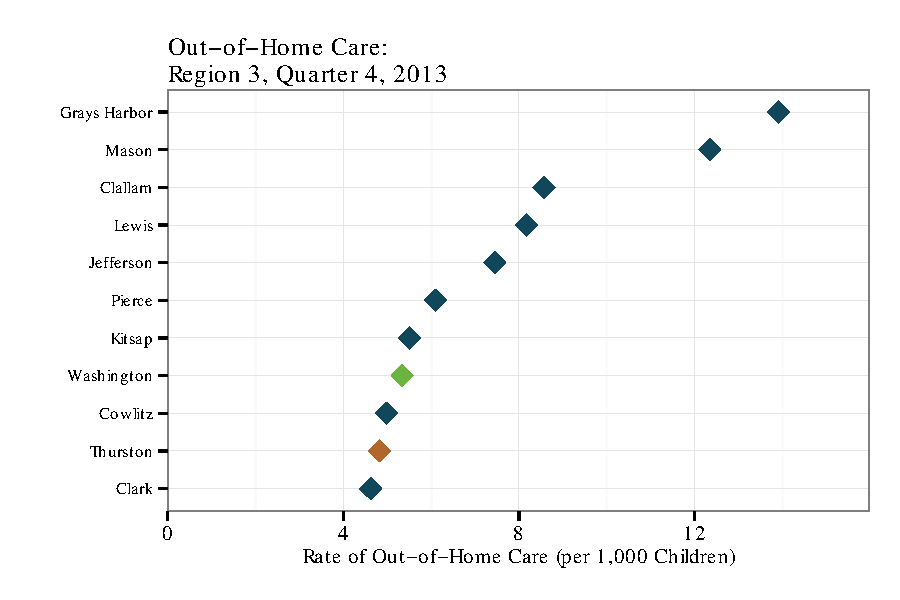
\includegraphics[width=\maxwidth]{figure/ooh_context} 

}



\end{knitrout}


\subsection{\href{http://www.partnersforourchildren.org/child-well-being/visualizations/out-home-care/safety}
    {Out-of-Home Care: Safety}
}

Sometimes when children experience a given permanency outcome (e.g., reunification, guardianship, adoption), safety concerns resurface in the child's home. In certain circumstances, these safety concerns are severe enough that the child needs to re-enter out-of-home care.

Table 3 identifies the percentage of children re-entering out-of-home care within two years of discharge, by discharge type, for all of the counties in 3, as well as for Washington State overall. Higher percentages of re-entery point to a difficulty of providing a permanent placement for the child (SENTENCE NEEDS WORK).


Blanks indicate that no children in the cohort exited to that discharge type, whereas 0\% indicates that children did exit to that discharge type, but none re-entered care.
\nopagebreak[4]
% latex table generated in R 3.0.0 by xtable 1.7-1 package
% Tue Apr 23 11:28:52 2013
\begin{table}[ht]
\centering
\begin{tabular}{rllll}
  \hline
 & County & Reunification & Adoption & Guardianship \\ 
  \hline
12 & Skamania & 42.9\% & 0\% &  \\ 
  6 & Jefferson & 37.5\% & 0\% & 0\% \\ 
  2 & Clallam & 31.8\% & 0\% & 0\% \\ 
  13 & Thurston & 22.2\% & 1.9\% & 11.1\% \\ 
  10 & Pacific & 16.7\% & 0\% & 0\% \\ 
  5 & Grays Harbor & 15\% & 0\% & 0\% \\ 
  11 & Pierce & 13.2\% & 2.1\% & 1.1\% \\ 
  3 & Clark & 13.1\% & 1.8\% & 4.3\% \\ 
  1 & Washington State & 12.8\% & 1.5\% & 5.7\% \\ 
  7 & Kitsap & 9.7\% & 0\% & 27.3\% \\ 
  9 & Mason & 8.8\% & 0\% & 0\% \\ 
  4 & Cowlitz & 6.9\% & 0\% & 0\% \\ 
  8 & Lewis & 6.5\% & 0\% & 33.3\% \\ 
  14 & Wahkiakum & 0\% &  &  \\ 
   \hline
\end{tabular}
\end{table}




%% Permanency Chunk

\end{document}

